\documentclass[mathserif]{beamer}
\usepackage{appendixnumberbeamer}
\usepackage[nofirafonts]{beamerthemefocus}
\usepackage{amsmath}
\usepackage{graphicx}
\usepackage{natbib}
\usepackage{floatrow}


\usepackage{xeCJK}
\setCJKmainfont{Iansui094-Regular}

\title{檢視中國債務陷阱\\Examining the Chinese Debt-Trap Diplomacy}
\author{陳家威\\{\small R10323045}}
\date{112年7月12日}

\begin{document}
    \begin{frame}
        \maketitle
    \end{frame}

    % \begin{frame}
    %     \frametitle{大綱}
    %         \begin{enumerate}
    %             \item 債務陷阱外交
    %             \item 中國貸款情形
    %             \item 主權債務違約模型
    %             \item 違約圖
    %             \item 結論
    %         \end{enumerate}
    % \end{frame}

    \section{債務陷阱外交}
    \begin{frame}
        \frametitle{出借99年的港口,與最空的機場}
        \begin{columns}
            \begin{column}{0.48\textwidth}
                    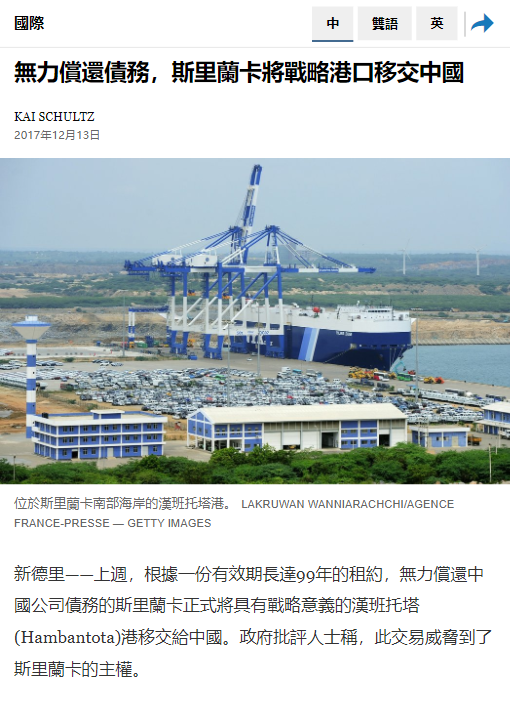
\includegraphics[width = \textwidth]{fig/Hambontota_news.png}
                    \footnotesize {圖片來源:紐約時報}
            \end{column}%
            \pause%
            \begin{column}{0.48\textwidth}
                    
\includegraphics[width = \textwidth]{fig/empty_airport.png}
                    \footnotesize {圖片來源:Forbes}
            \end{column}
        \end{columns}
    \end{frame}

    \begin{frame}
        \frametitle{一帶一路中的重要位置}
        \includegraphics<1>[width = \textwidth]{fig/BRI.png}%
        \includegraphics<2>[width = \textwidth]{fig/BRI_2.png}%
    \end{frame}

    \begin{frame}
        \frametitle{債務陷阱外交}
            \citet{Chellaney_2017} 首次提出
            \begin{block}{債務陷阱外交 Debt-trap Diplomacy}
               債權國刻意的向另一國提出大量的貸款,在債務國無法履行債務義務(多半是資產貸款,也可能包括基礎建設)時,強迫該國在經濟或是政治上的讓步。其貸款的條件多半不會公開,而貸款一般是用來支付給工程的承包商。\\
               The creditor country is said to extend excessive credit to a debtor country with the intention of extracting economic or political concessions when the debtor country becomes unable to meet its repayment obligations .
            \end{block}
    \end{frame}

    \section{中國貸款情形}

    \begin{frame}
        \frametitle{中國已正式成為全球最大債權國!}
        \centering
        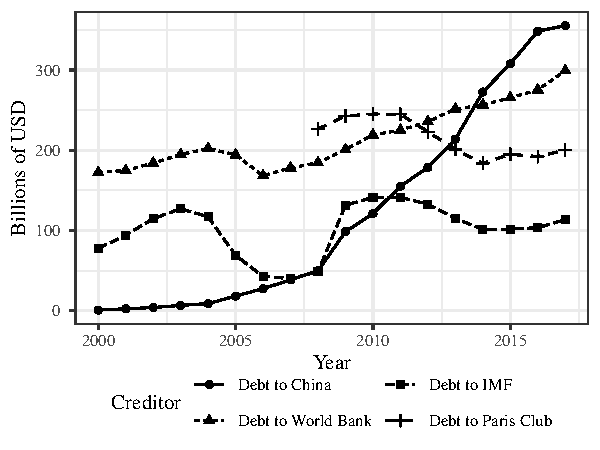
\includegraphics[width = 0.8\textwidth]{fig/aggr_debt_source.pdf}\\
        \small 資料來源:\citet*{Horn-Reinhart-Trebesch-21}
    \end{frame}

    \begin{frame}[label = {sri_ts}]
        \frametitle{中國借了斯里蘭卡多少錢?}
        \begin{center}
            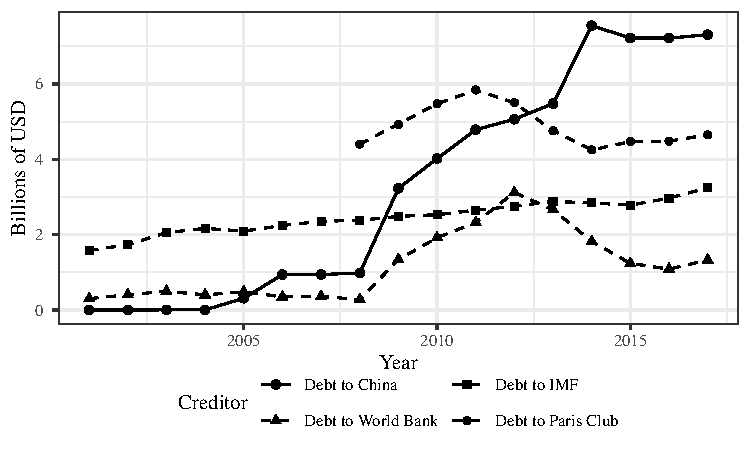
\includegraphics[width = 0.8\textwidth]{fig/ALL/Sri Lanka_debt_source.pdf}\\
            \small \hyperlink{sri_ds}{資料來源:}\citet*{Horn-Reinhart-Trebesch-21}
        \end{center}
    \end{frame}

    \begin{frame}[label = {pak_ts}]
        \frametitle{中國借了巴基斯坦多少錢?}
        \begin{center}
            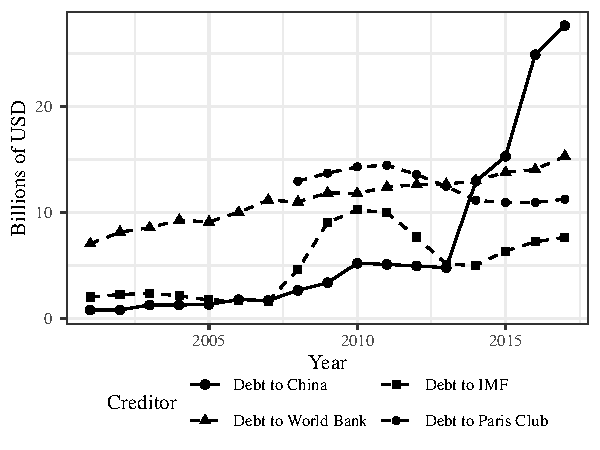
\includegraphics[width = 0.8\textwidth]{fig/ALL/Pakistan_debt_source.pdf}\\
            \small \hyperlink{pak_ds}{資料來源:}\citet*{Horn-Reinhart-Trebesch-21}
        \end{center}
    \end{frame}

    \begin{frame}
        \frametitle{中國是否借貸太多?}
            \begin{block}{債務陷阱外交 Debt-trap Diplomacy}
               債權國刻意的向另一國提出大量的貸款,在債務國無法履行債務義務(多半是資產貸款,也可能包括基礎建設)時,強迫該國在經濟或是政治上的讓步。其貸款的條件多半不會公開,而貸款一般是用來支付給工程的承包商。\\
               The creditor country is said to extend excessive credit to a debtor country with the intention of extracting economic or political concessions when the debtor country \textbf{becomes unable to meet its repayment obligations}.
            \end{block}
            \pause
            \vfill
            關鍵因素:使債務國還不出來 --- 違約
    \end{frame}

    \begin{frame}
        \frametitle{過去如何研究債務永續性?}
            大多研究著重在債務比例,無法直接回答「是否使債務國還不出來」
            \vfill
            \pause
            \begin{itemize}
            \item \citet{Hurley19-8-debt-trap}:樣本國家加入中國一帶一路債務之後,判斷債務占 GDP 有無增長,且超過50-60\%的臨界值,來判斷債務永續程度。
                \begin{itemize}
                    \item 臨界值根據 \citet{Chudik-15},為跨國臨界值面板 (cross-country panel threshold output growth model)
                \end{itemize}
            \item \citet{Bandiera-Vasileios-BRI-debt} 使用成長會計 (growth accounting) 估計 BRI 投資對GDP的影響,區分短期 / 長期受影響的國家。
            \end{itemize}
    \end{frame}

    \section{主權債務違約模型}
    \begin{frame}
        \frametitle{架構}
        \begin{itemize}
            \item 遵循 \citet{Hinrichsen_2020-chapter4}博士論文中的呈現方法 --- 違約圖 (Default Set Graph)
            \item 理論模型遵循 \citet*{Na-18} --- 競爭均衡下的違約模型
            \item 中國借貸資料:\citet*{Horn-Reinhart-Trebesch-21}
        \end{itemize}
    \end{frame}

    \begin{frame}
        \frametitle{主權債務違約模型}
        本研究參考\citet{Hinrichsen_2020-chapter4},採用 \citet{Na-18} 的模型
        \begin{itemize}
            \item 個體基礎的總體模型
            \item 當下狀態 + 評估未來終身價值 --- 決定違約
            \item 可得「最適違約區間」 Default set $D(d_t) = \left\{ y_t \mid v_c(y_t, d_t) < v_b(y_t) \right\}$
        \end{itemize}
    \end{frame}

    \begin{frame}[label = {vf}]
        \frametitle{政府決策過程}
        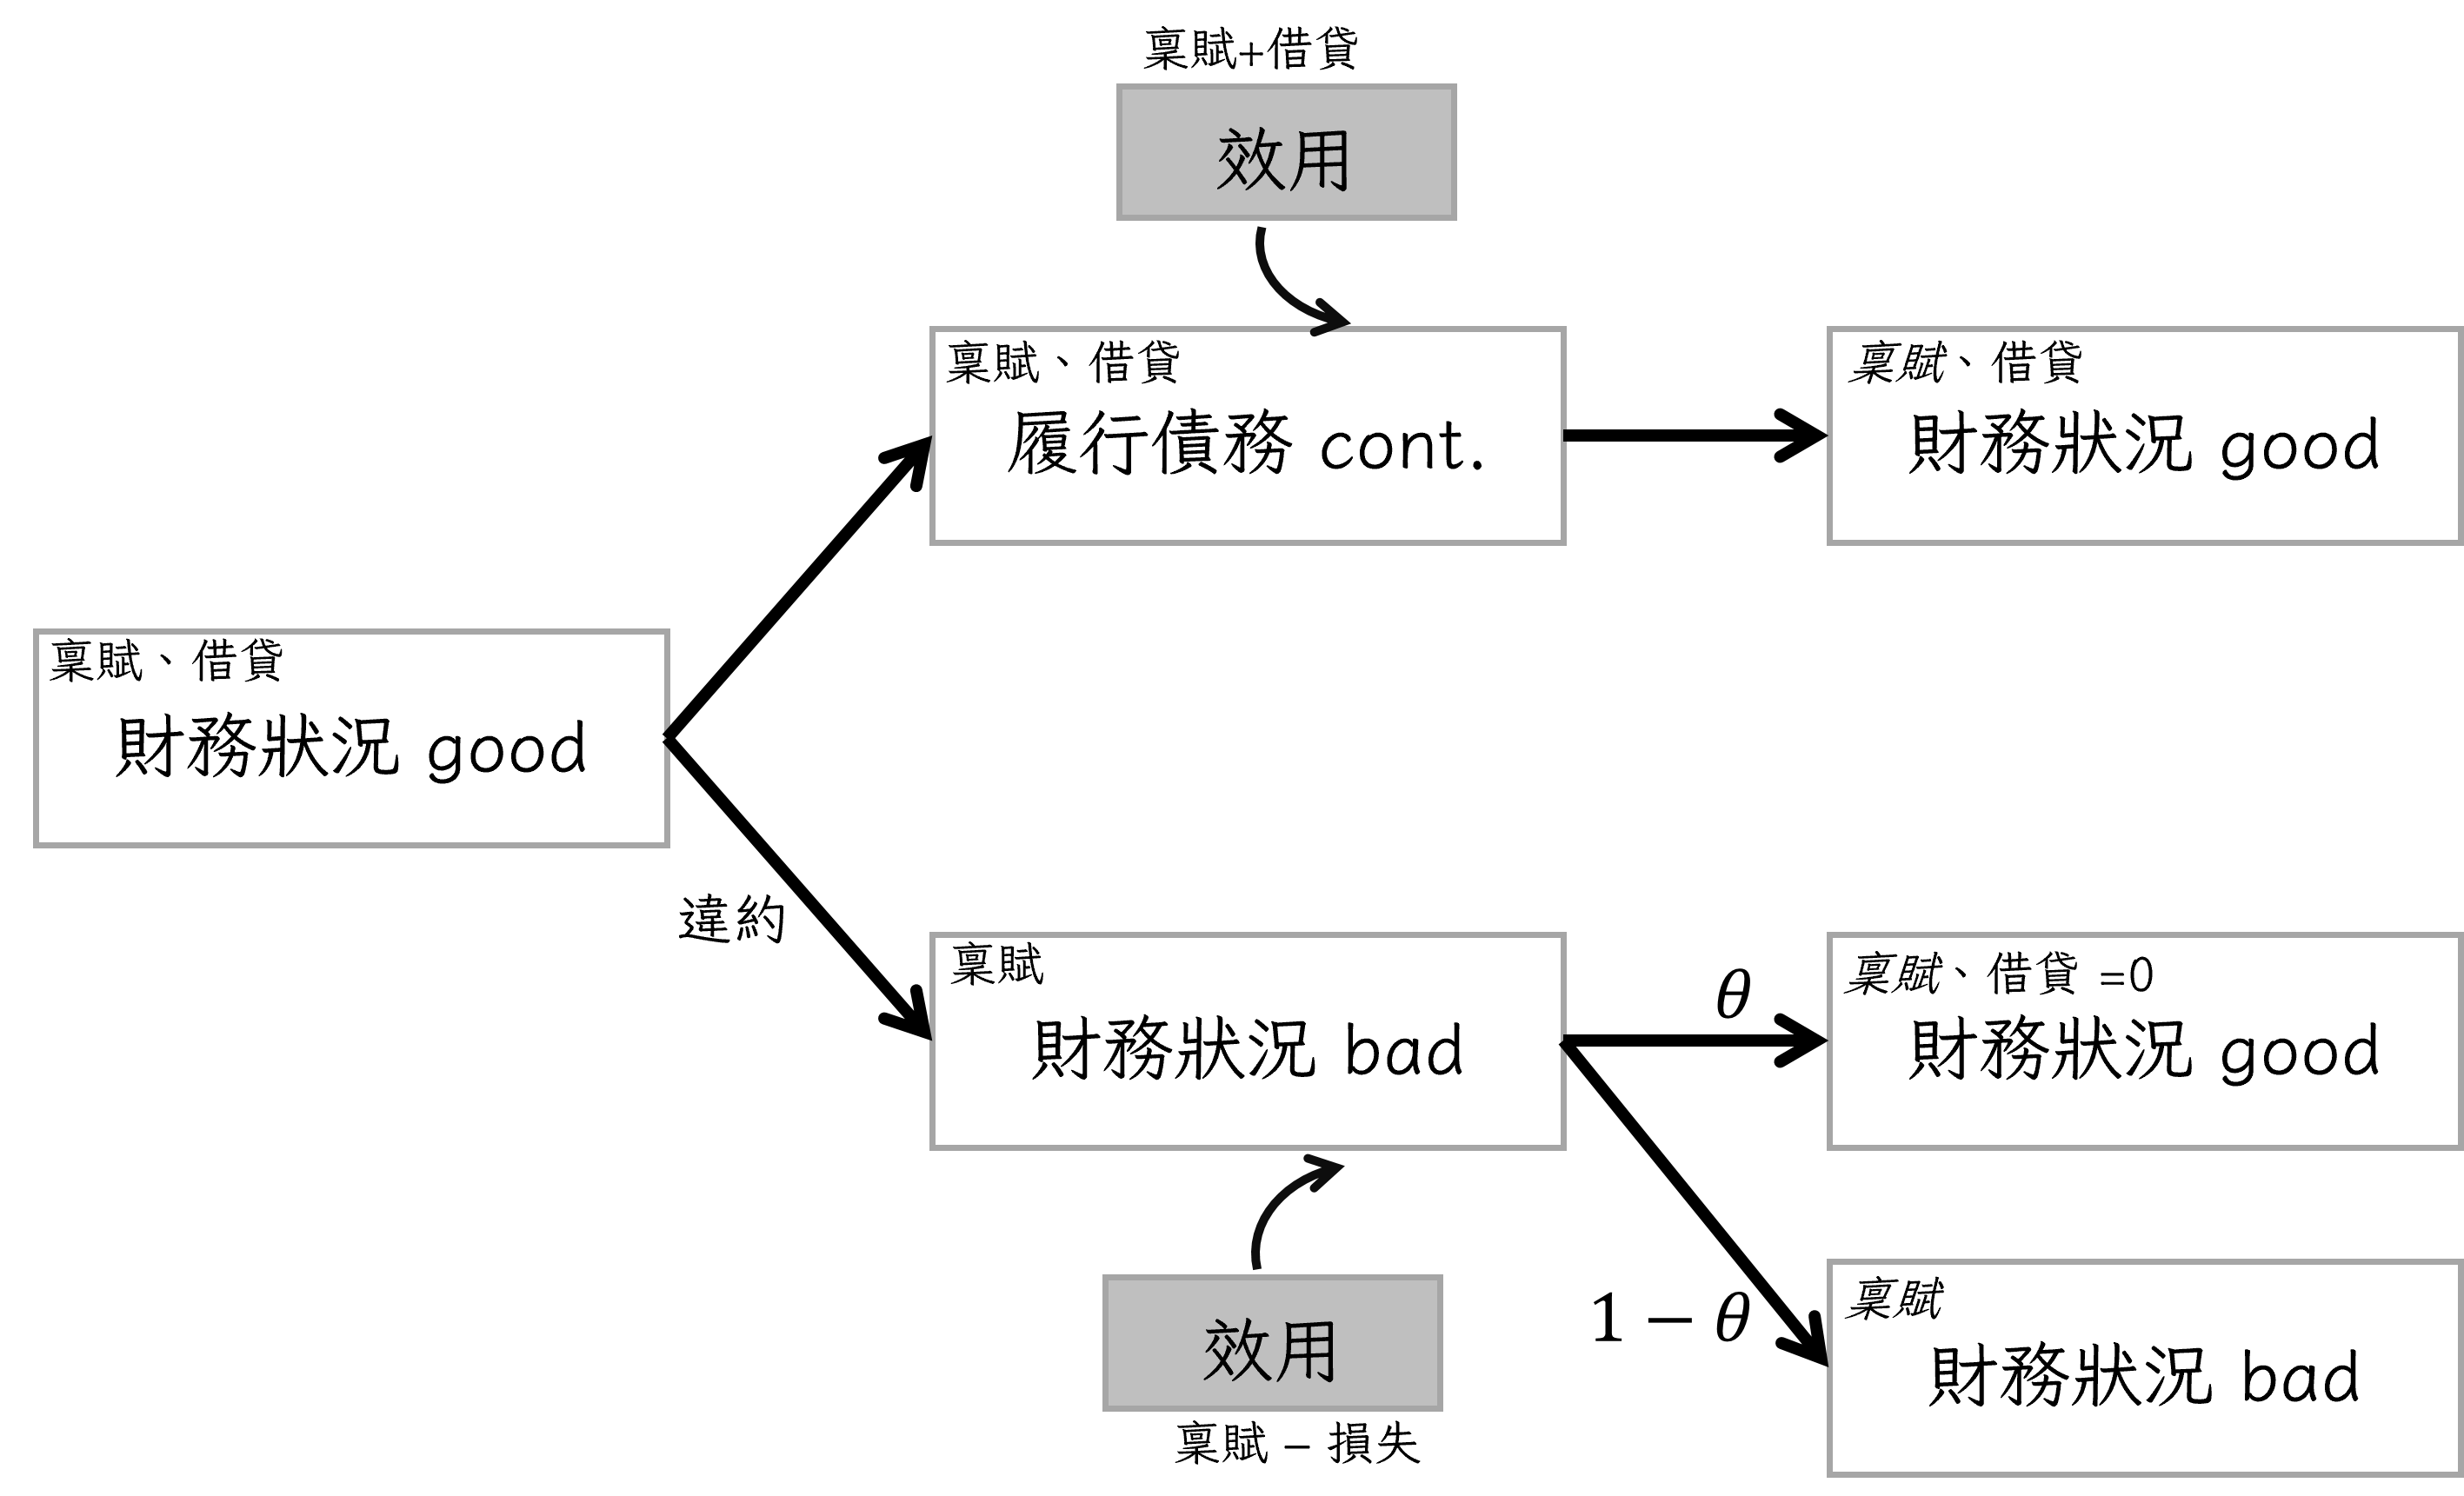
\includegraphics[width = \textwidth]{fig/value_fucntion_flow.png}
    \end{frame}

    % \begin{frame}
    %     \frametitle{模型刻劃 Calibration}
    %     \begin{itemize}[<+->]
    %         \item 勞動配額、可貿易產出占總產出比例、跨期消費替代彈性...等
    %         \item AR(1) 可貿易產出稟賦:人均實質可貿易 GDP $\rightarrow$ HP-Filter $\rightarrow$ 波動成分 $\rightarrow$ AR(1) 估計 $\rightarrow$ 持續性 + 波動性 $\rightarrow$ 轉移機率矩陣 (transition probability matrix)
    %         \item 時間偏好率\&損失函數的形式的選擇:讓模型產生符合三個均衡狀態
    %         \begin{itemize}
    %             \item 中國介入前的平均債務佔GDP比值 $\times$ haircut $\times$ 四季\footnote{模型假設全部違約,因此這個目標代表債務佔可貿易產出中會損失的比率}
    %             \item 一世紀平均違約次數
    %             \item 排除在金融市場外時,產出的損失
    %         \end{itemize}
    %     \end{itemize}
    % \end{frame}

    \section{違約圖}
    \begin{frame}
        \frametitle{由模型產生的違約圖 (Default Set)}
        斯里蘭卡為例 --- 灰色安全、白色違約:
        \begin{center}
        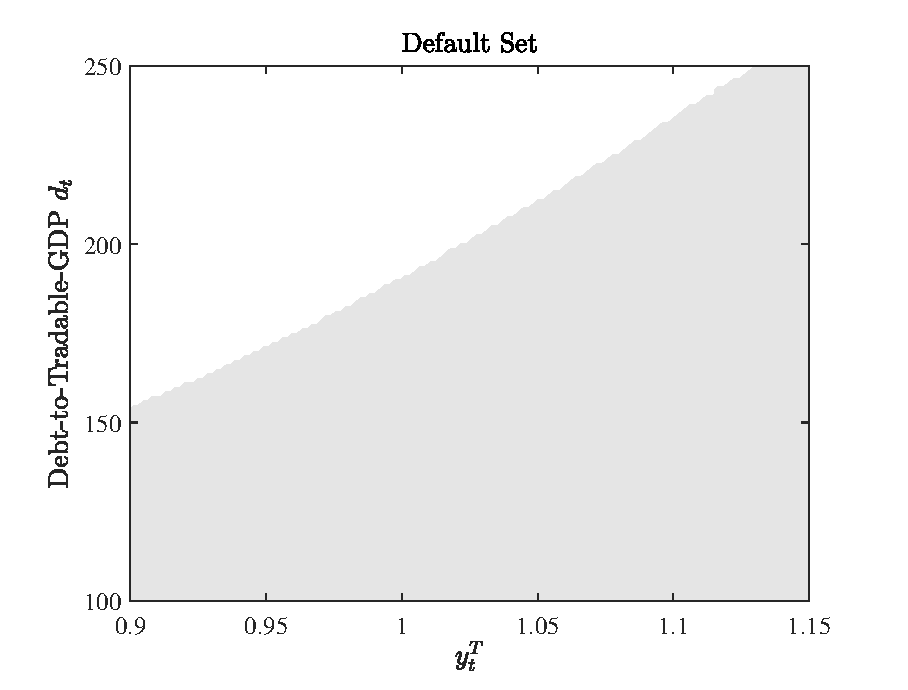
\includegraphics[height = 0.8\textheight]{fig/default_set_sri_trad_hp.eps}
        \end{center}
    \end{frame}

    \begin{frame}
        \frametitle{如何對應真實資料?}
        \pause
        \begin{itemize}
            \item<2-> $y^T_t$:使用去除趨勢之後的波動值 (Cyclical component)
            \item<3> $d_t$:總債務 / 名目可貿易 GDP $\times$ haircut $\times$ 4季
        \end{itemize}

        \only<2>{
            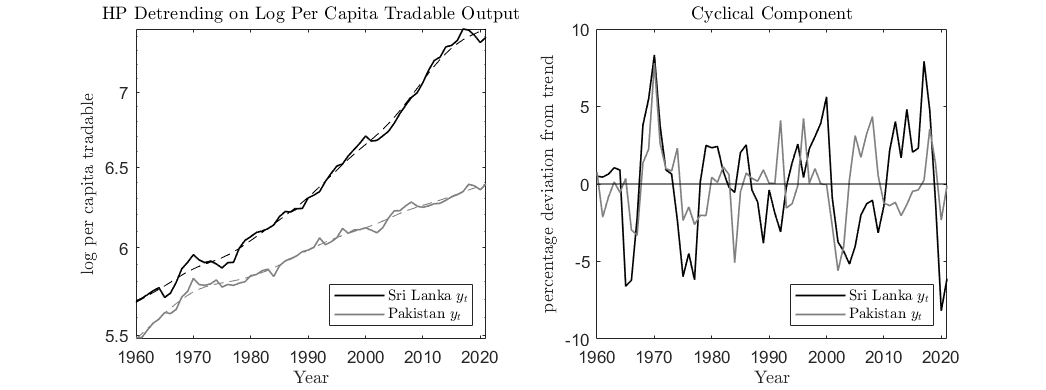
\includegraphics[width = \textwidth]{fig/decompose_trad_hp.png}
        }
        \only<3>{
        \begin{columns}
            \begin{column}{0.5\textwidth}
                \centering
                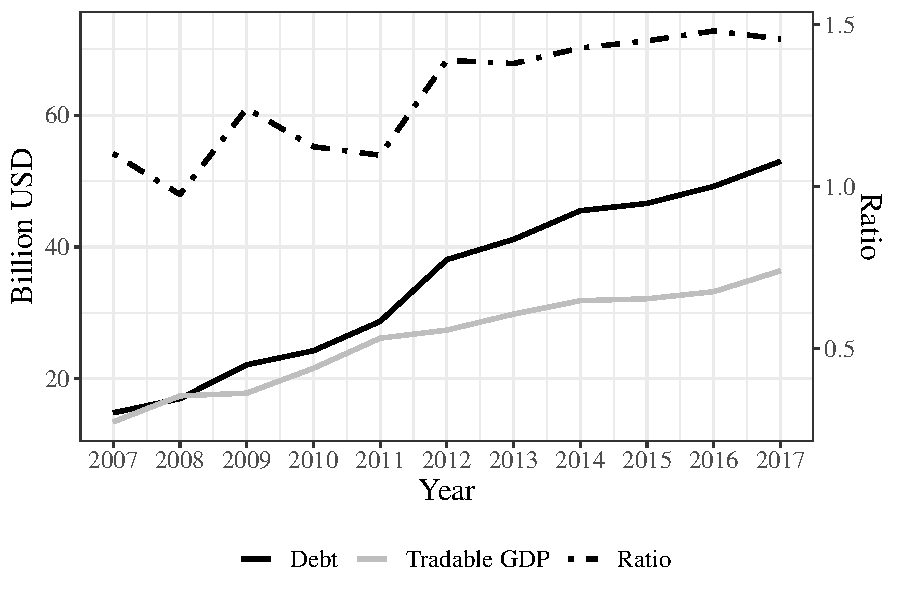
\includegraphics[width = \textwidth]{fig/sri_lanka_debt_gdp.pdf}
            \end{column}
            \begin{column}{0.5\textwidth}
                \centering
                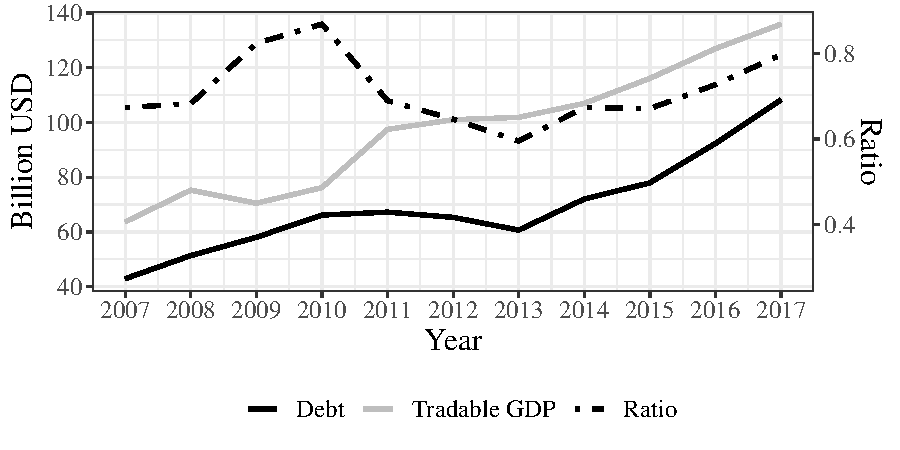
\includegraphics[width = \textwidth]{fig/pak_debt_gdp.pdf}
            \end{column}
        \end{columns}
        }
    \end{frame}

    \begin{frame}[label = {sri_ds}]
        \frametitle{斯里蘭卡有無被推向債務陷阱?}
        \centering
        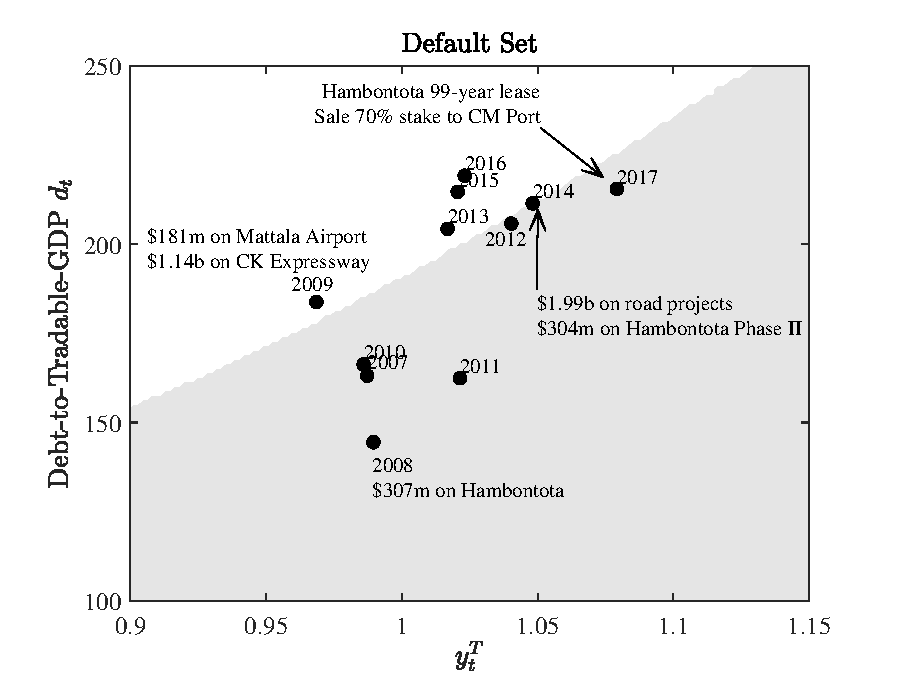
\includegraphics[width = 0.8 \textwidth]{fig/default_set_sri_trad_hp_with_china.eps}\\
        \hfill \hyperlink{sri_ts}{\tiny 斯里蘭卡債務時間軸}
    \end{frame}

    \begin{frame}[label = {pak_ds}]
        \frametitle{巴基斯坦有無被推向債務陷阱?}
        \centering
        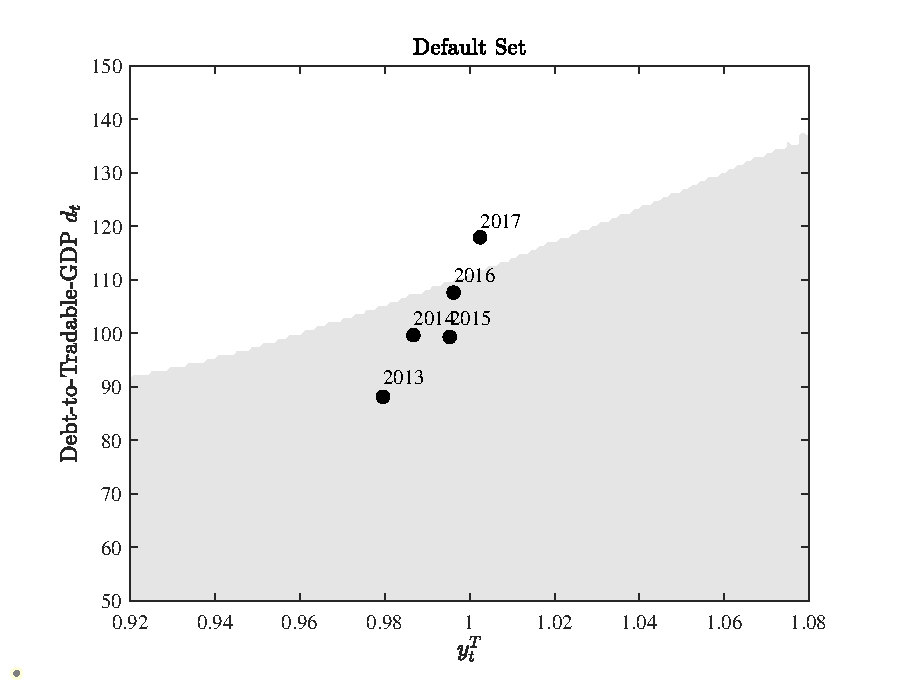
\includegraphics[width = 0.8 \textwidth]{fig/default_set_pak_trad_hp_with_china.eps}\\
        \hfill \hyperlink{pak_ts}{\tiny 巴基斯坦債務時間軸}
    \end{frame}

    \begin{frame}
        \frametitle{若移除中國的債務、還會違約嗎?}
        \centering
        \only<1-2>{斯里蘭卡\\}
        \only<3-4>{巴基斯坦\\}
        \includegraphics<1>[width = 0.8 \textwidth]{fig/sri_with_china.png}%
        \includegraphics<2>[width = 0.8 \textwidth]{fig/sri_x_china.png}%
        \includegraphics<3>[width = 0.8 \textwidth]{fig/pak_with_china.png}%
        \includegraphics<4>[width = 0.8 \textwidth]{fig/pak_x_china.png}%
    \end{frame}

    \begin{frame}
        \frametitle{兩種債務陷阱型態}

       \begin{enumerate}
        \item 原本沒有債務壓力,因接受過度借款而造成違約狀態。Ex:斯里蘭卡
        \item 過去早就有違約壓力,過度借款進一步惡化,最後又回到違約狀態。Ex:巴基斯坦
       \end{enumerate}

    \end{frame}
    \section{結論}
    \begin{frame}
        \frametitle{實證結果}

        \begin{enumerate}
            \item 本研究透過視覺化呈現結果,並提供一個客觀、可依循的流程,為檢視其他國家是否呈現「債務陷阱」提供操作型定義 (operational definition)
            \item 斯里蘭卡與巴基斯坦的確在中國介入之後,債務漸漸增高,進入違約區域,形成債務陷阱
            \item 從結果中可呈現出兩類型債務陷阱型態,為後續研究提供有關「債務陷阱」之敘述時,可遵循的特徵
        \end{enumerate}

    \end{frame}

    \begin{frame}
        \frametitle{限制及未來研究方向}
            \begin{enumerate}
                \item 模型的選擇 --- 受限於模型設定,「債務/GDP」、「排除金融市場期間」、「違約次數」等等的刻劃較不直觀 $\rightarrow$ 未來可使用考慮部分違約 (partial default) 的模型進行刻劃,如\citet{Bi-08}、\citet{Arellano-23-partial-default}等
                \item 一帶一路投資的影響 --- 本研究移除中國之債務時,並未考慮中國的投資對GDP的影響,因此容易高估去除中國的債務佔GDP比值。未來可延伸 \citet{Mendoza-Yue-12}並考慮在狀態變數中加入資本,以檢視資本衝擊的影響
            \end{enumerate}

    \end{frame}

    \begin{frame}[plain, noframenumbering]
        \begin{center}
            \Large
            謝謝聆聽!
        \end{center}    
    \end{frame}

    \appendix
    \begin{frame}[allowframebreaks]
            \frametitle{References}
            \bibliographystyle{econ}
            \bibliography{bib/ref}
    \end{frame}
\end{document}